\chapter{Calico}
This section provides an overview of Calico and the functionality it provided before improvements began. There were four main components that made up the core functionality of Calico. The four components were:

\begin{itemize}\itemsep1pt

\item
\textbf{Canvas \& Grid}. 
Canvases provided users with a basic sketching area where all interaction would take place. The grid provided an easy way for designers to organize and arrange different canvases.

\item
\textbf{Scraps}.
Scraps provided groups of content that could be easily interacted with. In the section below, these interactions are discussed in further detail.

\item
\textbf{Gestures}.
Gestures allowed designers to provide an easy way to interact with the board by performing specific commands. The gestures in Calico were meant to copy normal whiteboard interactions, such as using a fist to erase sketches, and slashing through scraps to delete them.

\item
\textbf{Palettes}.
The palette in Calico provides designers with a temporary storage area for commonly used components.


\end{itemize}

In the following sections, each component will be explained in more detail.


\section{Canvas \& Grid}

% http://en.wikibooks.org/wiki/LaTeX/Floats,_Figures_and_Captions
\begin{figure}[htb]
  \centering
  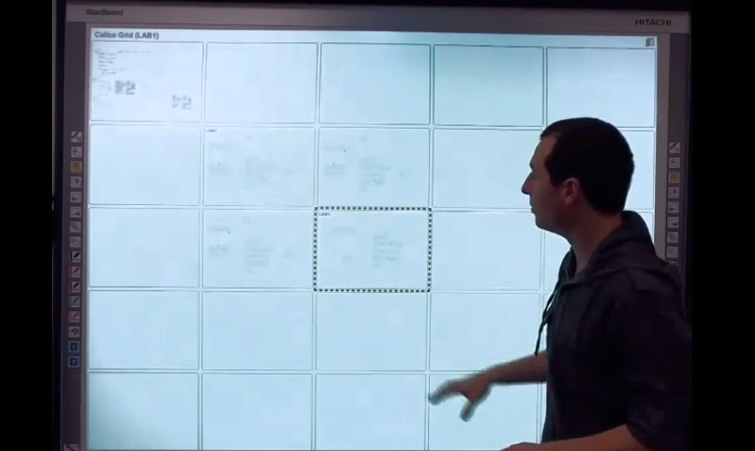
\includegraphics[width=0.8\textwidth]{grid.jpg}
  \caption{The grid view within Calico}
  \label{fig:grid}
\end{figure}

Designers not only need to keep track of their work, but they also need to constantly shift focus in their designs \cite{petre, zannier}.
The grid acts as an organizational tool for the sketches, and also allows designers to easily shift focus.
The grid, shown in Figure \ref{fig:grid}, organizes sketching areas in a row-column fashion, much like a spreadsheet organizes data. 
In Calico, ``canvases'' are used instead of cells which are used in a spreadsheet.
From the grid, designers can easily drag canvases and reposition them in different locations. This allows designers to logically organize their designs, as they can separate different designs (even completely different systems) from each other so that there is no confusion. 
The grid also allows designers to create a history of their design process by allowing them to create copies of existing canvases, so that their original design can be quickly compared with a new branch of thought. Each grid ``cell'' consists of a single sketching canvas. 
Users are able to freely sketch within each canvas, and canvases are kept separate from other canvases, so that designers can work uninterrupted. This means that designers working on unrelated designs can work using the same instance of Calico, but will not interfere with each other (the canvases can be kept completely separate no matter how many users are connected).
Each of these canvases can contain sketches, notes, or anything that the designer can draw on the canvas. 


\begin{figure}[h]
  \centering
  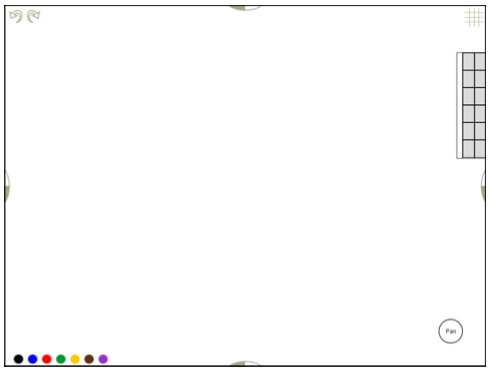
\includegraphics[width=0.6\textwidth]{blank_canvas.png}
  \caption{The default canvas view in Calico}
  \label{fig:canvas}
\end{figure}
Standard whiteboards do not easily allow designers to shift their focus quickly. This means that it is difficult for designers to create branches of their designs. If a designer wants to create a branch, they first need to duplicate their entire design elsewhere before they can edit it. The alternative would be to branch using the existing design, which would essentially destroy the previous design. Neither of these options is desirable as they lead to less design exploration -- hindering the design process. To remedy this problem, Calico has four gray tabs located on all edges of the sketching area (See Figure \ref{fig:canvas}). By clicking any one of the gray tabs, the entire contents of the current canvas is copied to the relevant adjacent canvas, and focus is then shifted to this newly created canvas. This allows designers to further explore an different design idea, but still allows them to revert to a previous state of their design. By repeatedly using tabs to create new design branches, a designer can develop a history of the evolution of their design. The designer essentially creates a ``filmstrip'' of activity that can serve as a timeline for the design \cite{filmstrip}. Using Calico's grid system, designers can arrange various canvases into groups that can be used to represent different concerns, or even separate ``old'' designs from newer ones.



\section{Scraps}

\begin{figure}[htb]
  \centering
  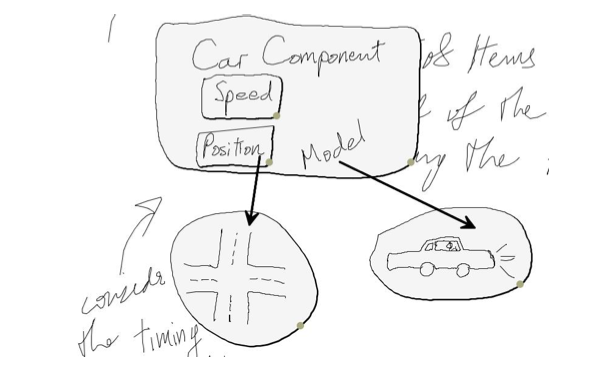
\includegraphics[width=0.8\textwidth]{scraps.png}
  \caption{Scraps (gray background) within Calico}
  \label{fig:scraps}
\end{figure}

Scraps in Calico can be thought of as ``scraps of paper'' that one would place on a desk or on a white board.
Scraps keep their shape -- whatever the designer draws, this shape will be kept throughout the design phase.
However, scraps are manipulatable in many different ways -- they are stackable, removable, relatable, and movable. 
For example, if a user drags a scrap and drops it on top of an existing scrap (that completely contains the respective scrap) then the smaller scrap will become attached to the larger scrap. This action ``stacks'' the scrap on top of another, and allows scraps to be easily grouped.
In the original version of Calico, all scraps have a ``dot'' that acts as a menu where various actions can be performed on the scrap itself.
In particular, a menu action was added that allows users to ``rectify'' a scrap -- convert it to the smallest rectangle that will contain any elements within the original scrap.
% Our goal is to be able to interact with the designers so that they are able to manipulate the objects, but we do not want to be intrusive in the way a formal design tool would be.

Scraps were created as the answer to allowing the content of a sketched design to become ``active'', while still allowing the designer to be free in their design.
As documented in Section 3, designers tend to use many different notations when they are designing. Thus, a tool like Calico should allow them to sketch in the notations that they are most comfortable with while still providing the advanced capability to manipulate a design at a higher level.
The key to this in Calico it leaves scraps in the same shape they were in when they were first drawn. 
As a result, the generic functionality is available for every shape, and designers can approximate a broad range of notations simply through shaping scraps.

Anything drawn on top of a scrap automatically becomes associated with that scrap.
Scraps can be placed on top of another scrap and the two will be ``stacked'' (as described above).
Designers can relate scraps with each other simply by drawing a line from one to the other, which would be converted to a directional arrow, linking the two scraps with each other. Scraps can also be dropped -- the entire contents of a scrap would be dropped to the element directly behind the scrap. If the scrap did not have anything behind it, then the content would be attached to the canvas.



\section{Gestures}
Many of the actions that Calico is designed to support require fluidity and speed of sketching. Calico should be as unobtrusive as possible to a designer. In order to be as unobtrusive as possible, common operations (such as erasing, or moving items) should be very easy to perform. The cost of making design changes has to be low \cite{petre}, so that designers are not impeded by the design software.

On one hand, menu-driven interaction greatly impedes the fluidity of the design process. On the other hand, allowing all operations to be accessible using gestures would require many complex gestures that would be very difficult for users to remember or perform. In an effort to reduce this effect, Calico uses mixed-mode interaction: commonly performed operations are available using gestures, while complex and less used operations are available via an easily accessible menu (the dot on the scraps). This reduces the number of gestures (and complexity of gestures), while still allowing the design process to be fluid.

Gestures in Calico are context-sensitive: they have different meanings depending on the situation and where the gesture is made on the canvas. 
For instance, a straight line can signal different things. 
If a line was drawn through a scrap, it was considered to be ``crossed out'' and the scrap (and any content contained within the scrap) would be deleted. 
If a line was drawn between two scraps then it was considered a relation, and an arrow was drawn linking the scraps to each other.
Once two scraps are linked, the arrow is then anchored to them, and would follow the scrap whenever it is moved on screen.

Another gesture that was added was the ability to enlarge a scrap by drawing a ``blister'' or bubble on the edge of the scrap.
By drawing this extra bubble, the scrap area would be enlarged to equal the size of the bubble that was just drawn. 
Users were also able to enlarge or shrink any arrow connecting two scraps. If they user made a pigtail motion over the arrow in a clockwise direction, then the arrow would be thickened. If the user drew the pigtail in a counter-clockwise direction, then the arrow would shrink.


\section{Palette}
The palette in Calico provides users with a ``drawer'' that can easily be used to store commonly used shapes and artifacts.
\begin{figure}[htb]
  \centering
  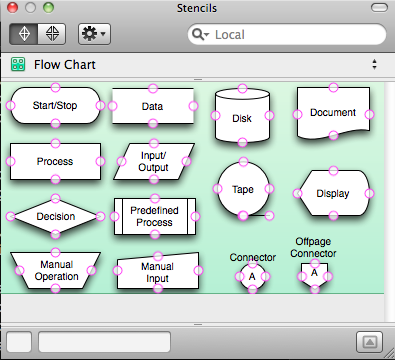
\includegraphics[width=0.5\textwidth]{palette.png}
  \caption{A container for commonly used components being used in OmniGraffle}
  \label{fig:palette_omnigraffle}
\end{figure}
The concept of a palette is something that can be seen in many current design programs. One example of this would be in OmniGraffle \cite{omnigraffle}. As shown in Figure \ref{fig:palette_omnigraffle}, its palette provides easy access to components that are commonly used during the design process. However, in most design tools this palette is populated with a predefined set of components, and this list cannot be modified by the designer. Due to the fact that Calico was designed to support the informal design process, it was decided that components in the palette should be determined by the designer. In Calico, the palette begins as a blank storage area that can be populated with content created by the designer, which allows for the reuse of sketched elements. 

The palette was designed to store scraps. To place a scrap into the palette, a designer simply need to drag the scrap into one of the available storage slots. The scrap (and any children of the scrap) would then be stored into the palette. The palette in Calico acted as a global storage area that was available on all canvases. This enabled designers to easily reuse components on different branches of design, or on completely different design sessions.  
